\documentclass[../IDP_Task5_Karwowski_Kowalewski.tex]{subfiles}

\begin{document} {
    This section contains results of compression single image ,,boat.png''. In order to explore and
    visualize results of compression process, the image was compressed mutliple times with many
    different parameter sets. 

    The two series of experiments were proccessed. Twe first series is related to 4x4 crop size, and
    the second series is related to 8x8 crop size. Each series constists of multiple compression
    attempts, which differ in number of neurons. Results of each series are presented in three
    figures: PSNR vs compression ratio plot, PSNR vs number of neurons plot and a compound figure
    containing thumbnails of all decompressed images from the series.

    \begin{figure}[!htbp]
        \centering
        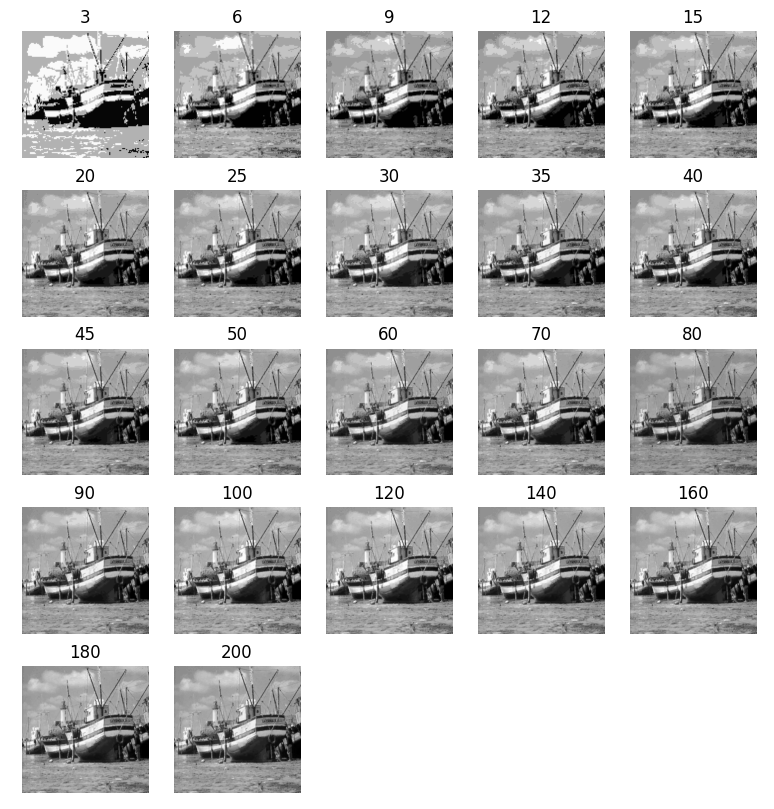
\includegraphics[width=\textwidth]{img/karwowski/4x4_images}
        \label{fig:4x4_images}
        \caption{Thumbnails of decompressed images with 4x4 crop size}
    \end{figure}
    
    \begin{figure}[!htbp]
        \centering
        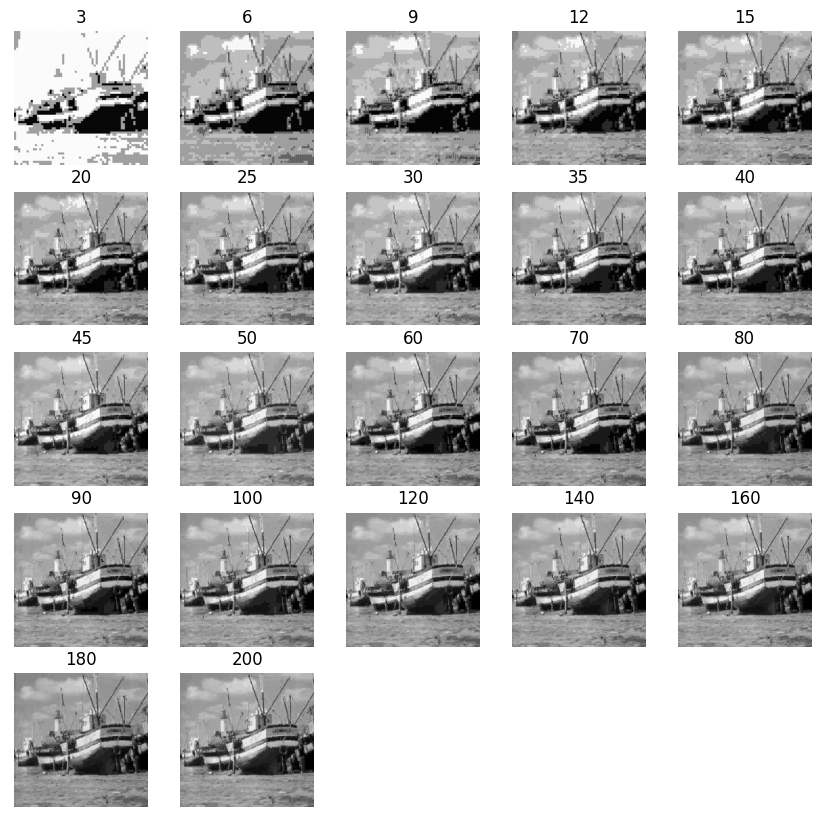
\includegraphics[width=\textwidth]{img/karwowski/8x8_images}
        \label{fig:8x8_images}
        \caption{Thumbnails of decompressed images with 8x8 crop size}
    \end{figure}

    \begin{figure}[!htbp]
        \centering
        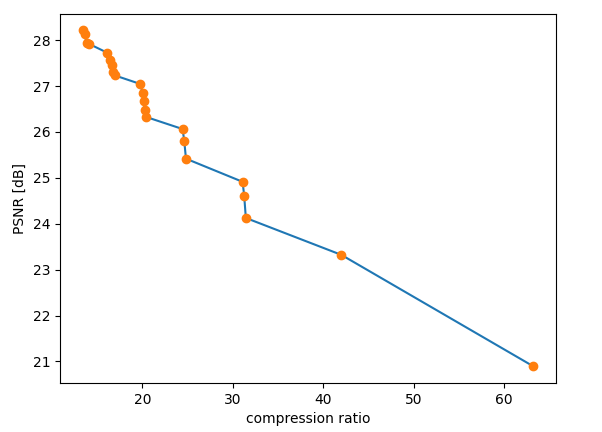
\includegraphics[width=\textwidth]{img/karwowski/4x4_compression_ratio}
        \label{fig:4x4_compression_ratio}
        \caption{PSNR vs compression ratio plot for 4x4 crop size}
    \end{figure}
    
    \begin{figure}[!htbp]
        \centering
        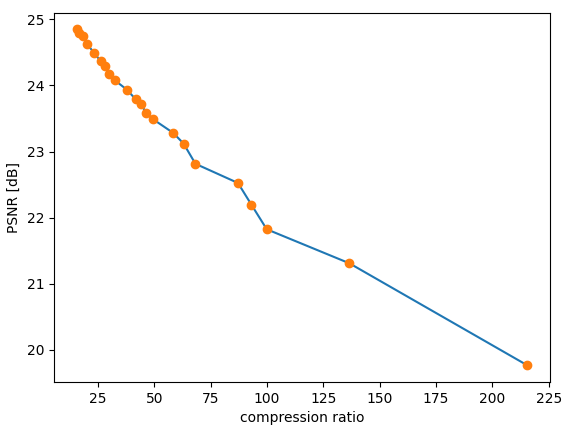
\includegraphics[width=\textwidth]{img/karwowski/8x8_compression_ratio}
        \label{fig:8x8_compression_ratio}
        \caption{PSNR vs compression ratio plot for 8x8 crop size}
    \end{figure}

    \begin{figure}[!htbp]
        \centering
        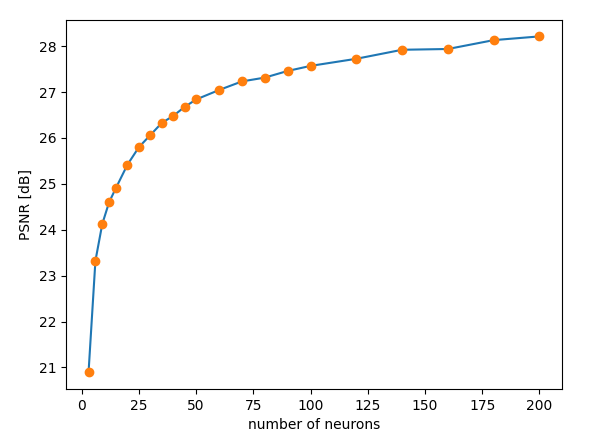
\includegraphics[width=\textwidth]{img/karwowski/4x4_number_of_neurons}
        \label{fig:4x4_number_of_neurons}
        \caption{PSNR vs number of neurons plot for 4x4 crop size}
    \end{figure}
    
    \begin{figure}[!htbp]
        \centering
        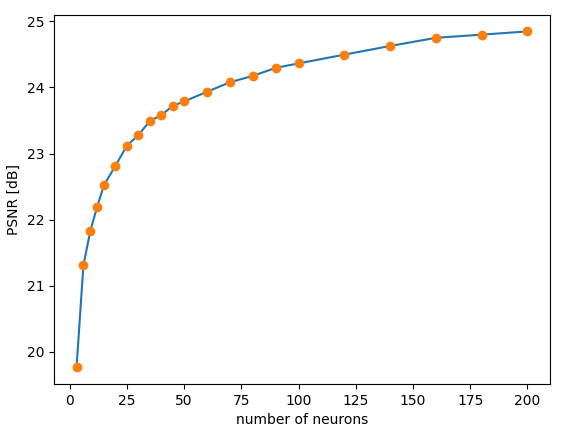
\includegraphics[width=\textwidth]{img/karwowski/8x8_number_of_neurons}
        \label{fig:8x8_number_of_neurons}
        \caption{PSNR vs number of neurons plot for 8x8 crop size}
    \end{figure}
    \FloatBarrier
}
\end{document}
